\section{Ranking of structural Ricardian comparative advantage }
In this section I present the results of the structural RCA ranking for both value-added exports measures and gross exports. First, I will first focus on the global view by highlighting the results of the association of the RCA ranking for gross exports and value-added exports against a country's per capita GDP. The hypothesis I focus is that country's with a higher GDP show a higher similarity between the rankings. Moreover, poorer countries production structure is such that sourcing and factor usage are more sector specific. \par Second, I will view at the structural RCA results by comparing the rankings for Belgium and Germany of forward and backward value-added exports to gross exports. In this way, I analyze whether two aspects, first whether value-added exports alter the picture of comparative advantage and whether the different perspectives of value-added exports show affect the results. 
\subsection{Structural Ricardian comparative advantage based gross exports and value-added exports}
I will discuss the choice of the association measures shortly. First, I chose the Spearman's $\rho$  since I focus on the similarity of rankings and the strength of the monotonic association between them. Moreover I chose Kendall's $\tau$ as it computes the similarity of the two rankings, by the means of counting the number of country pairs, which are different between two rankings.% Concretely, for each draw of country pairs I record in a binary variable, whether the draws are of the same order as in the ordered set. The binary variable is equal to one if the order is the same and zero else. In the next step I compute a simple correlation coefficient on the set of binary variables.     
\par 
I outline the construction of Kendall's $\tau$ here based on \textcite{abdi2007kendall}. The outline helps to provide the reason for the simple interpretation of Kendalls $\tau$ in terms of probabilities, which I will present after. The basic idea behind the measure is to count the number of different pairs for two sets of paired objects, which include the same objects  \textcite{abdi2007kendall}. I illustrate this idea in the context of the RCA rankings.  For two RCA rankings, the measure is based on counting the number of different country pairs, which I denote as $d(P_1, P_2)$, where $P_i \quad i=1,2$ indicates the order country ranking. In the next step, this number is normalized such that is bounded by -1 and 1, where -1 reflect the largest differences and 1 is equal to the smallest difference.  Kendall's $\tau$ is then defined as follows \[ \tau= \frac{1/2 N(N-1) - d(P_1,P_2)} {1/2 N(N-1)} \], %where the nominator $1/2 N(N-1)$ is equal to the number of pairs one can obtain from a set of $n$ objects. 
Moreover, Kendall $\tau$ has an intuitive stochastic interpretation \parencite{abdi2007kendall}. In the context of two country rankings, the interpretation is that if a country pair is randomly drawn from each ranking, Kendall's $\tau$ is equal to the difference between the probability that the draws are of the same order and the probability that the drawn country pairs are of a different order. The focus of Kendall's $\tau$ on country pairs is especially useful  for RCA, as the main focus of RCA is to compare the comparative advantage between pairs of countries and industries.   \par 
\begin{figure}[H]
\caption{Association RCA based on VAX \& EXGR and GDP per capita }
\centering
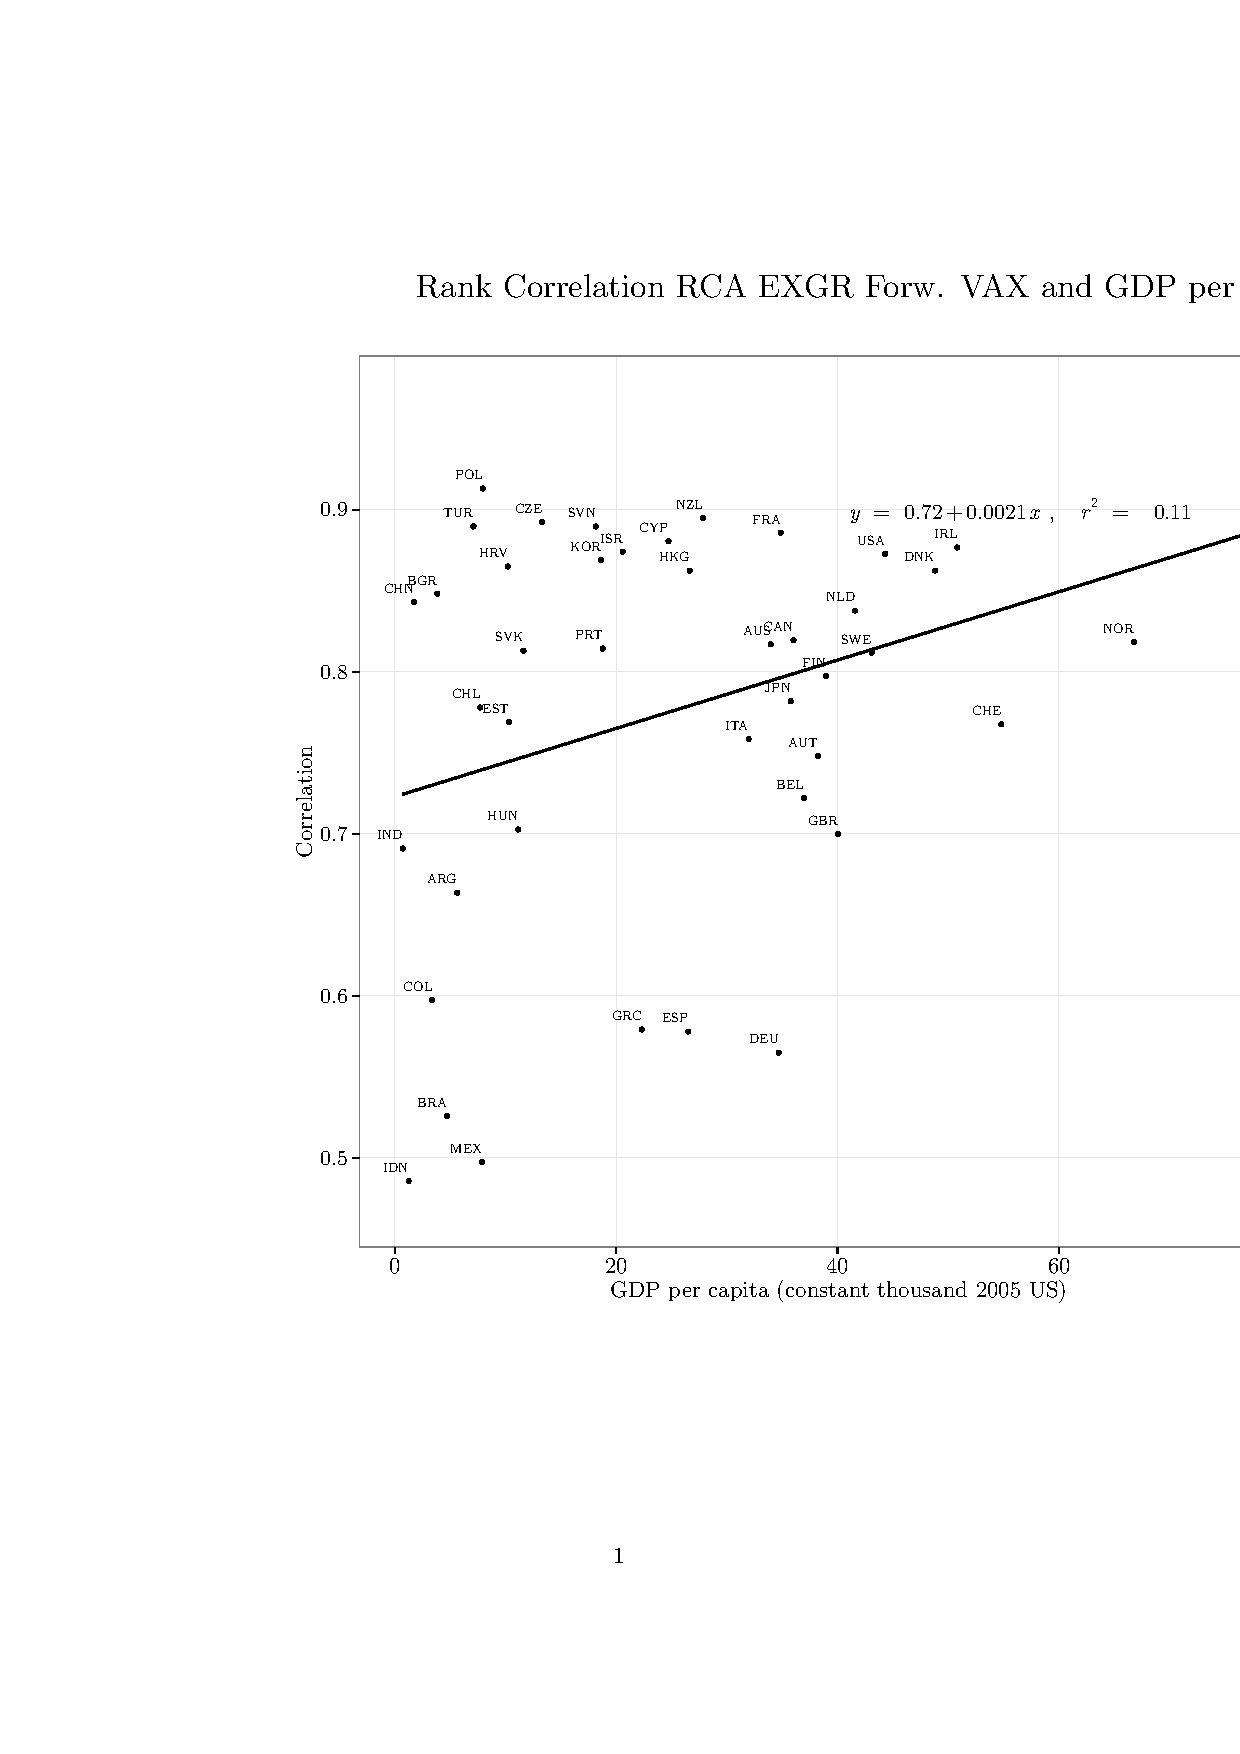
\includegraphics[width=.5 \linewidth]{./fig/spearman_fddva_std_balassa-march.tex}
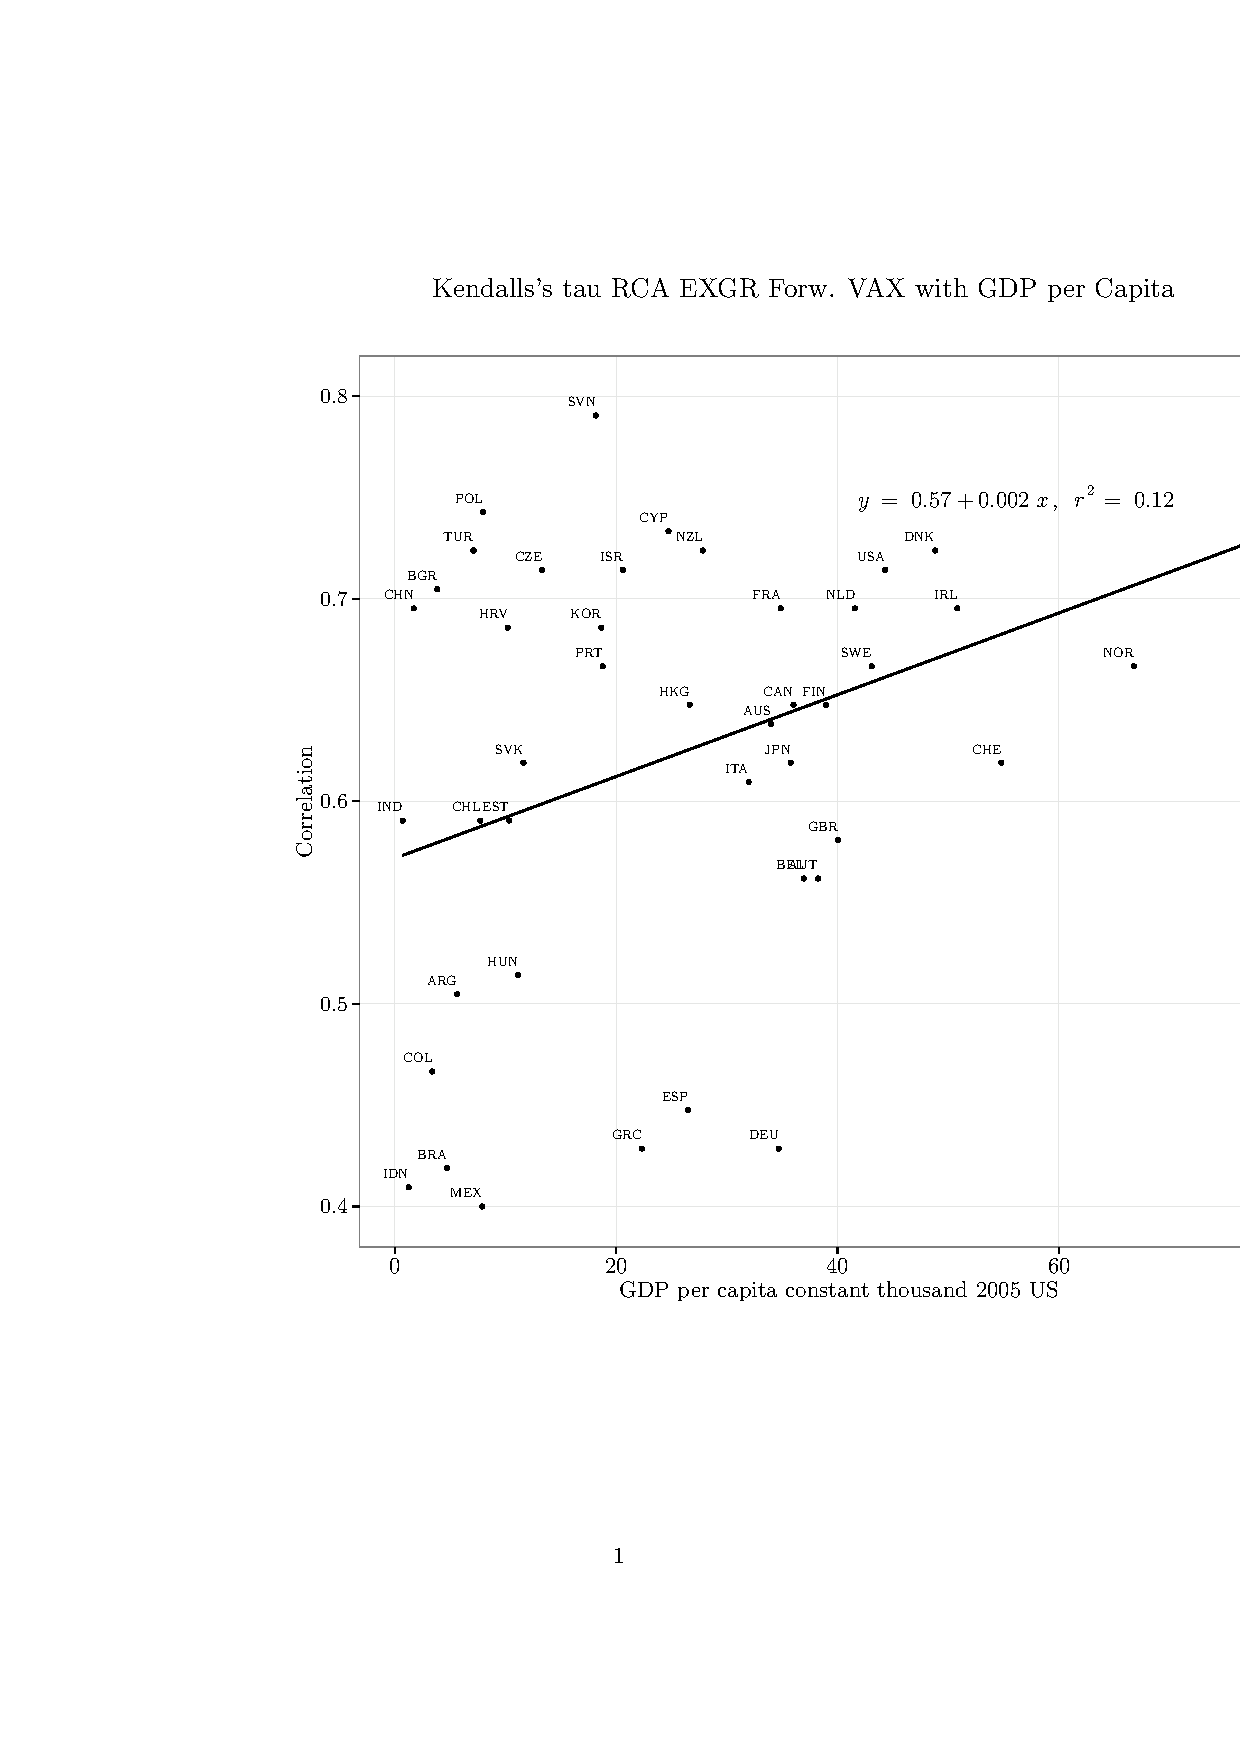
\includegraphics[width=.5 \linewidth]{./fig/kendall_fddva_exgr_std_balassa-march.tex}
 %\captionof{figure}{Another figure}
\end{figure}
I conclude two findings from the figures above. First, for both association measures I observe that there is a weak positive relation between the association measures and a country's gdp per capita measured in 2005 US dollar. Second, overall the Spearman rank correlation coefficients are higher compared to Kendall's $\tau$. The first finding  is consistent with the hypothesis that countries with a higher GDP have less sector specific input and sourcing patterns. The second finding is consistent with the result that asymptotically the ratio of the population analog of Spearman's $\rho$ and Kendall's $\tau$ is equal to three half \parencite{fredricks2007}. \par
Turning to the local view  I present below the normalized RCA based on both value-added export measures and gross exports.  I normalized the RCA \footenote{ RCA^k_{i}=\frac{z^k_i* \bar{z}}{\bar{z_i} *\bar{z^k}}, where \bar{z�} denotes the grand mean, \bar{z^k} denotes the sector specific mean and \bar{z_i} denotes the country specific mean} as in \texcite{leromain2014}, such that a value above 1 indicates a comparative advantage of the country in the particular industry. I will first discuss the results for backward value-added exports and gross exports. \par 
 
\begin{figure}
\caption{Country pair RCA based on for- and backward  VAX \& EXGR }
\includegraphics[width=.5\linewidth]{./fig/forw_exgr_DEU_BEL_tiva.tex}
\includegraphics[width=.5\linewidth]{./fig/back_exgr_DEU_BEL_tiva.tex}
\end{figure}

\endinput